\chapter{The $3x+1$ Problem}\label{chap:intro}

Take a positive integer. If it is even, halve it; if it is odd, triple it and
add one. Repeat. Starting from $7$ the sequence runs
\[
  7,\ 22,\ 11,\ 34,\ 17,\ 52,\ 26,\ 13,\ 40,\ 20,\ 10,\ 5,\ 16,\ 8,\ 4,\ 2,\ 1,
\]
and once it reaches $1$ it falls into the loop $1\to4\to2\to1$ forever. The
$3x+1$ problem asks whether this always happens. Every starting value that
anyone has ever tried, and the number of starting values tried is now
$2^{71}$, eventually reaches $1$. Nobody knows why.

The problem can be explained to a child and has defeated some of the strongest
mathematicians of the last ninety years. It sits at an unusual junction. The
rule is arithmetic, but the behaviour it produces looks random; the obvious
probabilistic heuristic predicts the answer with great accuracy, but the
heuristic is not a proof and no one knows how to turn it into one; and
generalizations of the problem that look only slightly more complicated are
provably undecidable. This book is about that junction, read through the lens
of martingales\index{martingale}, optimization and Diophantine\index{Diophantine approximation} approximation. This first chapter
states the problem, recounts its history, works through examples, surveys what
is known, and lays out the plan of the book.

\section{The conjecture}\label{sec:ch1:conjecture}

We write $\N=\{1,2,3,\ldots\}$ for the positive integers. The \emph{standard
Collatz map} $T_0:\N\to\N$ is
\begin{equation}\label{eq:ch1:T0}
  T_0(n)=\begin{cases} n/2, & n \text{ even},\\ 3n+1, & n \text{ odd}.\end{cases}
\end{equation}
We write $T_0^{(k)}$ for the $k$th iterate, with $T_0^{(0)}(n)=n$, and call the
sequence $n, T_0(n), T_0^{(2)}(n),\ldots$ the \emph{orbit} or
\emph{trajectory} of $n$.

\begin{conjecture}[The Collatz conjecture]\label{conj:ch1:collatz}
For every $n\in\N$ there is $k\geq0$ with $T_0^{(k)}(n)=1$.
\end{conjecture}

The least such $k$ is the \emph{total stopping time\index{stopping time}} of $n$, written
$\sigma_\infty(n)$, with the convention $\sigma_\infty(n)=\infty$ if no such
$k$ exists. The conjecture says $\sigma_\infty(n)<\infty$ for every $n$.

It is useful to see at once what could go wrong. The orbit of $n$ is a sequence
of positive integers, so exactly one of three things happens.
\begin{enumerate}[label=(\roman*),leftmargin=2em]
\item The orbit reaches $1$, and from then on cycles through $1,4,2$.
\item The orbit is unbounded: $\limsup_k T_0^{(k)}(n)=\infty$. Since the orbit
  cannot revisit a value without becoming periodic, in this case all its
  values are distinct and in fact $T_0^{(k)}(n)\to\infty$.
\item The orbit is bounded but never reaches $1$. A bounded orbit takes only
  finitely many values, so it must eventually repeat a value, and then it is
  periodic from that point on. Hence the orbit enters a cycle that does not
  contain $1$.
\end{enumerate}
The conjecture is the assertion that alternatives (ii) and (iii) never occur.
We shall call these the \emph{divergence half} and the \emph{cycle half} of
the problem. They look like two aspects of one question, but one of the main
messages of this book is that they are different in kind and call for
different tools.

That the problem is genuinely arithmetic, and not a consequence of some soft
principle about tripling and halving, is shown by running the same rule on the
negative integers\index{negative cycles}. Formula \eqref{eq:ch1:T0} makes sense on all of $\Z$, and
there it has at least three cycles besides the fixed point $0$: the cycle
$-1\to-2\to-1$, the cycle
\[
  -5\to-14\to-7\to-20\to-10\to-5,
\]
and a cycle of length $18$ through $-17$, containing $7$ odd terms, whose most
negative value is $-272$. On the negative integers the conjecture is therefore
false, in the sense that there is more than one cycle. Notice the counts: the
cycle through $-5$ has $2$ odd steps and $3$ halvings, and $2^3<3^2$; the
cycle through $-17$ has $7$ odd steps and $11$ halvings, and $2^{11}<3^{7}$.
For the trivial positive cycle, $1$ odd step and $2$ halvings, the inequality
is reversed: $2^2>3$. We shall see in \cref{chap:cycles} that a positive cycle
with $r$ odd steps and $s$ halvings must satisfy $2^s>3^r$ with
$s\log2-r\log3$ extremely small, which is a statement about rational
approximations $s/r$ to $\lt$. The fractions $3/2$ and $11/7$ that appear in
the negative cycles approximate $\lt=1.58496\ldots$ from below.

\paragraph{Variants of the map.} Since $3n+1$ is even whenever $n$ is odd, one
loses nothing by combining each tripling with the halving that must follow it.
This gives the \emph{accelerated map\index{accelerated map}} $T(n)=(3n+1)/2$ for odd $n$ and
$T(n)=n/2$ for even $n$. Going further, one may divide out all factors of $2$
at once, which gives the \emph{Syracuse map\index{Syracuse map}} $S(n)=(3n+1)/2^{\vt(3n+1)}$ on odd
integers, where $\vt(m)$ is the exponent of the largest power of $2$ dividing
$m$. The three maps are equivalent for the conjecture, and each is the natural
object for some purpose. \cref{chap:parity} sets them side by side; for now we
work with $T_0$, which is the map in the statement.

\section{A brief history}\label{sec:ch1:history}

The problem is usually attributed to Lothar Collatz\index{Collatz, L.}, who studied iterations of
simple arithmetic functions as a student in Germany in the 1930s and is said
to have recorded problems of this type in his notebooks then. He did not
publish it. The problem was in circulation by the early
1950s~\cite[pp.~3 to 4]{lagarias1985} and spread by word of mouth for
decades, and as it
travelled it collected names. Helmut Hasse\index{Hasse, H.} lectured on it, and it became known
as \emph{Hasse's algorithm}; it reached Syracuse University, and became the
\emph{Syracuse problem}; Shizuo Kakutani\index{Kakutani, S.} circulated it at Yale and Chicago,
and it became \emph{Kakutani's problem}; Stanislaw Ulam\index{Ulam, S. M.} spread it at Los
Alamos and elsewhere, and it became \emph{Ulam's problem}. It is also called
the $3x+1$ problem, the $3n+1$ problem, and the Collatz problem, the name we
use. The multiplicity of names is itself a historical record: the problem was
rediscovered or relayed by many people before anyone wrote about it in print.

The standard account of the history is the survey of
Lagarias\index{Lagarias, J. C.}~\cite{lagarias1985} in the \emph{American Mathematical Monthly},
which is still the best introduction to the mathematics. Lagarias recounts Kakutani's remark that
for about a month everybody at Yale worked on the problem without result, and
he records Paul Erd\H{o}s\index{Erdos, P.@Erd\H{o}s, P.}'s verdict: ``Mathematics is not yet ready for such problems.''
Erd\H{o}s offered a prize for a solution, and the remark
has been quoted ever since, sometimes as a warning and sometimes as a
challenge. We take it as a description of the situation. The tools that have
produced partial results, namely density arguments, stochastic models,
Diophantine\index{Diophantine approximation} approximation and $2$ adic dynamics, are each strong enough to
explain why the conjecture should be true and each falls short of proving it
for a reason that can be stated precisely, and a large part of this book states those reasons.

The literature has grown large. Lagarias has maintained annotated
bibliographies~\cite{lagarias2003bib,lagarias2006bib} covering the work from
1963 onward, and he edited the volume \emph{The Ultimate
Challenge}~\cite{lagarias2010}, published by the American Mathematical Society
in 2010, which collects survey articles on the history, the stochastic models,
the computational verification, the generalizations, and the connections with
ergodic theory and logic, together with reprints of key papers. The reader who
wants a single reference besides this book should start there. The research
monograph of Wirsching\index{Wirsching, G. J.}~\cite{wirsching1998} treats the problem as a dynamical
system and is a second good entry point.

\section{Worked orbits}\label{sec:ch1:orbits}

The best way to feel the problem is to compute. Every number quoted in this
section was computed by the authors with the scripts listed in
\cref{app:code}.

\begin{example}[The orbit of $27$]\label{ex:ch1:27}
Small starting values usually reach $1$ quickly: $3$ takes $7$ steps, $7$ takes
$16$ steps and climbs to $52$, $9$ takes $19$ steps. The value $27$ is the
first surprise. Its orbit begins
\[
\begin{gathered}
  27,\ 82,\ 41,\ 124,\ 62,\ 31,\ 94,\ 47,\ 142,\ 71,\\
  214,\ 107,\ 322,\ 161,\ 484,\ 242,\ 121,\ 364,\ \ldots
\end{gathered}
\]
and wanders upward for a long time. It reaches its maximum $9232$ at step $77$
and finally arrives at $1$ after $\sigma_\infty(27)=111$ steps under $T_0$.
Of these $111$ steps, $41$ are triplings and $70$ are halvings.
\cref{fig:ch1:orbit27} shows the whole orbit on a logarithmic scale.
\end{example}

\begin{figure}[t]
\centering
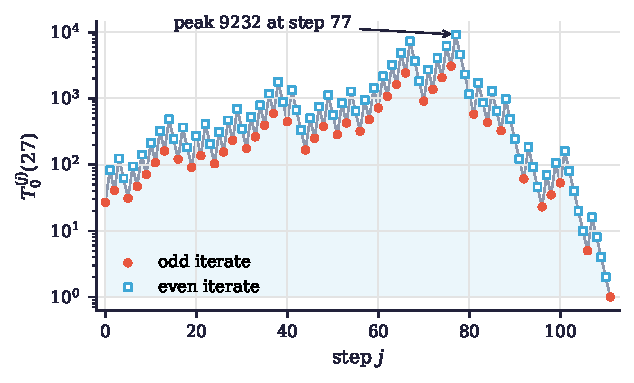
\includegraphics[width=\textwidth]{figures/ch1_orbit27.pdf}
\caption{The orbit of $27$ under the standard map $T_0$, on a logarithmic scale. Iterates are marked by parity: every odd iterate $x$ is followed by a rise to $3x+1$ and every even iterate by a halving, so the odd iterates are the points where the path turns upward. The orbit takes $111$ steps to reach $1$ and peaks at $9232$ after $77$ steps.}
\label{fig:ch1:orbit27}
\end{figure}

The counts in this example already contain most of the arithmetic we shall
need. Because each tripling is followed by at least one halving, the same orbit
takes $111-41=70$ steps under the accelerated map\index{accelerated map} $T$ and $41$ steps under the
Syracuse map\index{Syracuse map} $S$. Each tripling multiplies by slightly more than $3$ and each
halving divides by exactly $2$, so an orbit with $41$ triplings and $70$
halvings that starts at $27$ and ends at $1$ must have $27\cdot3^{41}$ a little
below $2^{70}$. Indeed $27\cdot3^{41}/2^{70}\approx0.834$, and the gap from
$1$ is made up by the additive ones. We make this exact in
\cref{chap:parity}, where we show that $2^k T^{(k)}(n)=3^m n+c_k(n)$ under
the accelerated map, with $m$ the number of odd steps among the first $k$ and
$c_k(n)$ an explicit integer, positive as soon as $m>0$, built from the
positions of the odd steps.

The orbit of $27$ is also a reminder that orbits merge. The orbit of $97$
reaches $94$ after $13$ steps; the orbit of $27$ reaches $94$ after $6$ steps;
from $94$ onward the two coincide. Hence $\sigma_\infty(97)=13+105=118$ and
the orbit of $97$ peaks at $9232$ as well.
The orbits that reach $1$ form a tree rooted at $1$, once the edge from $1$ to $4$ is removed; it is a component of the \emph{Collatz graph}, which joins each $n$ to $T_0(n)$, and the conjecture says that this tree contains every positive integer.

\paragraph{Records.} A starting value $n$ is a \emph{delay record} if
$\sigma_\infty(n)>\sigma_\infty(n')$ for every $n'<n$. The delay records up to
$10^5$ are
\[
\begin{aligned}
&1,\,2,\,3,\,6,\,7,\,9,\,18,\,25,\,27,\,54,\,73,\,97,\,129,\,171,\,231,\\
&313,\,327,\,649,\,703,\,871,\,1161,\,2223,\,2463,\,2919,\,3711,\\
&6171,\,10971,\,13255,\,17647,\,23529,\,26623,\\
&34239,\,35655,\,52527,\,77031.
\end{aligned}
\]
\cref{tab:ch1:records} lists a selection with their total stopping times\index{stopping time} and
peaks. The longest orbit below $10^4$ starts at $6171$ and takes $261$ steps;
below $10^5$ it starts at $77031$ and takes $350$ steps; below $10^6$ it starts
at $837799$ and takes $524$ steps. Peaks can be enormous relative to the
starting value: below $10^4$ the highest point reached by any orbit is
$27\,114\,424$, from $n=9663$, and below $10^5$ it is $1\,570\,824\,736$, from
$n=77671$.

\begin{table}[t]
\centering
\caption{Selected delay records for the standard map $T_0$: total stopping
time $\sigma_\infty(n)$ and the largest value in the orbit.}
\label{tab:ch1:records}
\begin{tabular}{@{}rrr@{}}
\toprule
$n$ & $\sigma_\infty(n)$ & $\max_k T_0^{(k)}(n)$ \\
\midrule
$7$ & $16$ & $52$ \\
$9$ & $19$ & $52$ \\
$27$ & $111$ & $9\,232$ \\
$97$ & $118$ & $9\,232$ \\
$871$ & $178$ & $190\,996$ \\
$6\,171$ & $261$ & $975\,400$ \\
$77\,031$ & $350$ & $21\,933\,016$ \\
$837\,799$ & $524$ & $2\,974\,984\,576$ \\
\bottomrule
\end{tabular}
\end{table}

\paragraph{How long do orbits take?} \cref{fig:ch1:totalstop} plots
$\sigma_\infty(n)$ for all $n\leq10^5$ against $\log n$. Two features stand
out. The points fill a band whose centre grows linearly in $\log n$, and the
band is wide, with a visible fine structure of streaks caused by merging
orbits. The linear growth is predicted by the simplest probabilistic model.
Under $T_0$ an odd value is always followed by an even one, and on average
about one step in three is odd. If we pretend that the parities are random
with $\Prob(\text{odd})=1/3$, each step changes $\log x$ by $\log3$ (ignoring
the $+1$) with probability $1/3$ and by $-\log2$ with probability $2/3$, so the
mean change per step is
\[
  \tfrac13\log3-\tfrac23\log2=\tfrac13\log\tfrac34\approx-0.0959.
\]
An orbit starting at $n$ should therefore need about
\[
  \frac{3\log n}{\log(4/3)}\approx10.43\log n
\]
steps, which is the line drawn in the figure.
The least squares line through the origin fitted to $\sigma_\infty(n)$ against $\log n$ over $2\leq n\leq10^4$ has slope $10.36$, and over the range $2\leq n\leq10^5$ of \cref{fig:ch1:totalstop} it has slope $10.23$.
For the accelerated map, whose heuristic slope is $2/\log(4/3)=1/|\ds|\approx6.952$ with $\ds=\log(\sqrt3/2)$, the fitted slopes over the same two ranges are $6.920$ and $6.837$.
The constant
$\ds$ will be a central character in \cref{chap:stochastic}.

\begin{figure}[t]
\centering
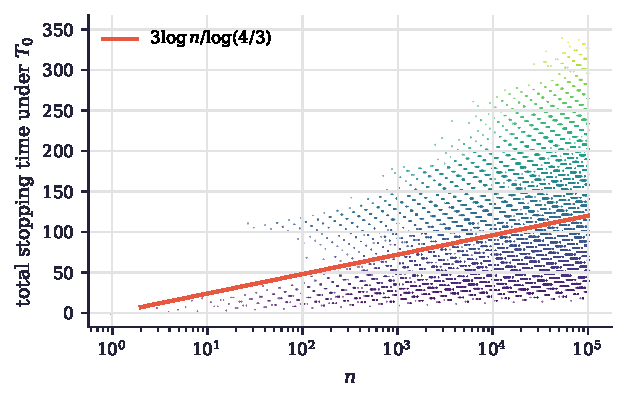
\includegraphics[width=\textwidth]{figures/ch1_totalstop.pdf}
\caption{Total stopping times $\sigma_\infty(n)$ under $T_0$ for all $n\leq10^5$, with $n$ on a logarithmic scale. The solid line is the prediction $3\log n/\log(4/3)$ of the random parity model. The streaks are families of starting values whose orbits merge after a few steps.}
\label{fig:ch1:totalstop}
\end{figure}

The agreement between heuristic and computation is good, and it is worth
being clear about what it does and does not mean.
It is consistent with the parities of the accelerated map along a typical orbit having the frequencies of fair coin flips, so that one step of $T_0$ in three is odd.
It does not
mean that any particular orbit must descend, and it gives no handle at all on
the question of whether some exceptional orbit could avoid $1$ forever. The
heuristic averages over starting values, while the conjecture is about every
starting value. That gap recurs in every chapter of this book.

\section{Computational verification}\label{sec:ch1:verification}

Because the conjecture is a universal statement about integers, it invites
computation, and the problem has been checked by computer for almost as long
as there have been computers. Each verification establishes that every $n$ up
to some bound $X$ reaches $1$. The techniques are clever: one need only check
that each $n$ eventually falls below itself, since smaller values have already
been handled; residue classes that provably fall below their starting value in
a few steps can be skipped wholesale, which is the idea behind the stopping
time analysis of \cref{chap:parity}; and the accelerated and Syracuse forms
let one take several steps at once using precomputed tables indexed by
residues modulo a power of $2$.

The bounds have grown by many orders of magnitude. In the 2000s Oliveira e Silva\index{Oliveira e Silva, T.}
verified the conjecture up to $5\cdot2^{60}\approx5.76\times10^{18}$, an effort
described in his chapter of the Lagarias\index{Lagarias, J. C.} volume~\cite{oliveira2010}. In 2021
Ba\v{r}ina\index{Barina, D.@Ba\v{r}ina, D.}~\cite{barina2021} reported verification up to $2^{68}\approx
2.95\times10^{20}$, using a carefully optimized algorithm on graphics
processors, and in 2025 he extended it to
$2^{71}\approx2.36\times10^{21}$~\cite{barina2025}. Most of the computations
in this book use the range $2^{68}$: whenever we say \emph{the verified range\index{verification range}} we
mean that every $n\leq2^{68}$ is known to reach $1$. We shall see that the
sharp form of the cycle bound below is the same at $2^{71}$.

Verification has two consequences beyond the obvious one. First, any orbit
that fails to reach $1$ must stay above $2^{68}$ forever, because if it ever
dropped to $2^{68}$ or below it would join a verified orbit. In particular a
nontrivial cycle would have least element above $2^{68}$. Second, and less
obviously, this lower bound on the least element can be converted into a lower
bound on the length of a cycle, by an argument going back to
Crandall\index{Crandall, R. E.}~\cite{crandall1978} and
Eliahou\index{Eliahou, S.}~\cite{eliahou1993} that uses the continued fraction\index{continued fraction} of $\lt$. In
\cref{chap:cycles} we carry out this argument in detail.
A first version, the block form of the bound, which uses only the convergents\index{convergent} of $\lt$, shows that with the verified range $2^{68}$ every nontrivial cycle contains at least $6\,586\,818\,670$ odd terms.
A sharper version, which uses a short mediant lemma\index{mediant lemma} together with the classical description of the best one sided approximations~\cite[Theorem~4.5(ii)]{hancl2019}, both proved in \cref{chap:cycles}, to show that the extremal cases always occur at intermediate fractions\index{semiconvergent} of the continued fraction lying above $\lt$,
gives unconditionally
\[
  r\;\geq\;72\,057\,431\,991
\]
for the number $r$ of odd terms in any nontrivial cycle. It coincides with the
bound $r>7.2\times10^{10}$ that Hercher\index{Hercher, C.}~\cite{hercher2023} credits to
Hercher and Puchert\index{Puchert, S.}~\cite{hercher2018,puchert2018}. Applied to Eliahou's
verification range $2^{40}$, the same method returns exactly his lower bound
$17\,087\,915$ on the length of a cycle of the accelerated map\index{accelerated map}. The
current record is larger still: Hercher~\cite[Corollary~29]{hercher2023}
showed, by a sharper accounting of the structure of a cycle, that verification
up to $1536\cdot2^{60}=3\cdot2^{69}$ gives $r\geq1.375\times10^{11}$, and
Ba\v{r}ina's verification to $2^{71}$~\cite{barina2025} has made this
unconditional. Cycles, if they exist, are very long and live very
high up.

Verification can never prove the conjecture, and it is not even clear what
evidential weight it carries. Orbits that misbehave, if they exist, might
start at numbers so large that no computation will ever reach them. The
heuristic of \cref{sec:ch1:orbits} predicts that the longest orbits below $N$
take time of order $\log N$, so nothing in the data suggests a change of
regime, but one should remember that the problem has a large supply of
quantities that grow like $\log N$ or $\log\log N$, and phenomena governed by
such quantities can hide far beyond the reach of any computer.

\section{Undecidability: Conway's theorem}\label{sec:ch1:conway}

Why should such a simple problem be hard? One answer is that the class of
problems it belongs to contains problems that are not merely hard but
impossible. In 1972 Conway\index{Conway, J. H.}~\cite{conway1972} considered \emph{generalized
Collatz maps}: fix a modulus $p\geq2$ and rational numbers $a_0,\ldots,a_{p-1}$
and $b_0,\ldots,b_{p-1}$, chosen so that
\[
  g(n)=a_i n+b_i \qquad\text{whenever } n\equiv i\pmod p
\]
maps integers to integers. The Collatz map is the case $p=2$, $a_0=1/2$,
$b_0=0$, $a_1=3$, $b_1=1$. Conway showed that this class is rich enough to
simulate any computation: given a Turing machine one can construct such a $g$
whose iterates encode the steps of the machine. It follows that there is no
algorithm which, given $g$ in this class and a starting value $n$, decides
whether the orbit of $n$ under $g$ eventually reaches $1$. Conway's
construction in fact needs only the maps with all $b_i=0$, which multiply by a
rational depending on the residue class.

Conway later packaged this observation as a programming language,
FRACTRAN\index{FRACTRAN}~\cite{conway1987}. A FRACTRAN program is a finite list of fractions
$q_1,\ldots,q_t$; the state is a positive integer $n$; one step replaces $n$ by
$q_i n$ for the first $i$ such that $q_i n$ is an integer, and the program halts
if there is none. Each such step is a generalized Collatz map with all $b_i=0$
and modulus the least common multiple of the denominators. Conway exhibited a
FRACTRAN program of fourteen fractions whose orbit starting at $2$ passes
through exactly the powers of $2$ with prime exponent, in increasing order,
and showed that FRACTRAN is a universal model of computation. Kurtz\index{Kurtz, S. A.} and
Simon\index{Simon, J.}~\cite{kurtz2007} sharpened the logical classification, showing that the
generalized problem of deciding whether every orbit of a given $g$ reaches $1$
is complete for the class $\Pi^0_2$ of the arithmetic hierarchy.

None of this says that the original problem is undecidable, and indeed a
single statement such as \cref{conj:ch1:collatz} is either true or false; the
undecidability concerns algorithms that work uniformly over the whole class.
What Conway's theorem does say is that any proof of the Collatz conjecture\index{Collatz conjecture}
must use something specific about the numbers $2$ and $3$. Soft arguments
that would apply equally to every map of the form $a_i n+b_i$ cannot work,
because for some maps in the class the corresponding statement is false, and for every sound, recursively axiomatized theory there are maps for which it is true but not provable in that theory.
This is the
theoretical counterpart of the observation about negative integers\index{negative cycles} above.
In this book the specific arithmetic of $2$ and $3$ enters in three places:
the Geometric law of $\vt(3n+1)$ in \cref{chap:parity}, through the comparison of its mean $2$ with $\lt$ (the same law holds for $\vt(5n+1)$, but $\log_25>2$), the identity
$\tfrac12\cdot\tfrac12+\tfrac12\cdot\tfrac32=1$ behind the martingale\index{martingale} of
\cref{chap:stochastic}, and the continued fraction\index{continued fraction} of $\lt$ in
\cref{chap:cycles}.

\section{What is known: density theorems}\label{sec:ch1:density}

Since proving the conjecture for every $n$ is out of reach, a natural weakening
is to prove it for almost every $n$, in some sense of density. Recall that a
set $A\subseteq\N$ has \emph{natural density} $\delta$ if
$\#\{n\leq x:n\in A\}/x\to\delta$ as $x\to\infty$, and \emph{logarithmic
density} $\delta$ if
\[
  \frac{1}{\log x}\sum_{n\leq x,\ n\in A}\frac1n\;\longrightarrow\;\delta .
\]
Natural density $1$ implies logarithmic density $1$, but not conversely, so
logarithmic density statements are weaker.

\paragraph{Terras and Everett.} The first theorem of this type concerns the
\emph{stopping time\index{stopping time}} $\sigma(n)$, the least $k\geq1$ with $T^{(k)}(n)<n$ under
the accelerated map\index{accelerated map}. Terras\index{Terras, R.}~\cite{terras1976,terras1979} and, independently,
Everett\index{Everett, C. J.}~\cite{everett1977} proved that the set of $n$ with $\sigma(n)<\infty$
has natural density $1$. Terras proved more: for each $k$ the set
$\{n:\sigma(n)\leq k\}$ has a natural density $F(k)$, and $F(k)\to1$. The key
idea, common to both, is that the first $k$ parities of the orbit of $n$ depend only on $n$
modulo $2^k$, and that every pattern of $k$ parities occurs for exactly one
residue class~\cite[Theorem~B]{lagarias1985}. We prove all of this in \cref{chap:parity}, where it is
\cref{thm:terras} and \cref{thm:density}. A stopping time result is weaker than
it looks: it says that almost every orbit eventually goes below its starting
value, which, applied repeatedly, does not show that almost every orbit reaches
$1$, because the exceptional set at each stage could catch the orbit.

\paragraph{Smaller and smaller.} Later work showed that almost all orbits go
much lower. Korec\index{Korec, I.}~\cite{korec1994} proved that for every
$\theta>\log3/\log4\approx0.7925$ the set of $n$ whose orbit contains a value
below $n^{\theta}$ has natural density $1$. The exponent $\log3/\log4$ has the
same source as the drift\index{drift} $\log(3/4)$ of the Syracuse map\index{Syracuse map} that we compute in
\cref{chap:parity}.

\paragraph{Krasikov and Lagarias.} A different kind of result counts the
integers that are known to reach $1$. Writing $\pi_1(x)$ for the number of
$n\leq x$ whose orbit contains $1$, Krasikov\index{Krasikov, I.} and Lagarias\index{Lagarias, J. C.}~\cite{krasikov2003}
proved, by a system of difference inequalities\index{difference inequality} derived from the structure of
the Collatz graph modulo powers of $3$, that $\pi_1(x)\geq x^{0.84}$ for all
sufficiently large $x$. This is far from density $1$, but it is a statement
about orbits that actually reach $1$, not merely orbits that descend.

\paragraph{Tao.} The strongest result to date is due to Tao. For the smallest
value attained by the orbit of $n$ under the standard map\index{standard map} we write
\[
  \mathrm{Col}_{\min}(n)=\min_{k\geq0}T_0^{(k)}(n).
\]

\begin{theorem}[{Tao~\cite[Theorem~1.3]{tao2022}}]\label{thm:ch1:tao}
Let $f:\N\to\R$ be any function with $f(n)\to\infty$ as $n\to\infty$. Then
\[
  \mathrm{Col}_{\min}(n)<f(n)
\]
for all $n$ in a set of logarithmic density $1$.
\end{theorem}

Taking $f(n)=\log\log\log\log n$, for example, the theorem says that almost
every orbit, in logarithmic density, eventually dips below
$\log\log\log\log n$. This is the sense of the title of Tao\index{Tao, T.}'s paper: almost all
orbits attain almost bounded values. It is a remarkable strengthening of the
Terras and Korec results, which give the weaker bounds
$\mathrm{Col}_{\min}(n)<n$ and
$\mathrm{Col}_{\min}(n)<n^{\theta}$. The proof works with the Syracuse map. Its
deep input is a fine scale mixing
estimate~\cite[Proposition~1.14]{tao2022}: the residues modulo powers of $3$ of the
Syracuse iterates of a suitably random starting value are governed by a certain
\emph{Syracuse random variable} that encodes the first few Syracuse steps, and
this variable is approximately equidistributed\index{equidistribution} at fine $3$ adic scales,
although far from uniform at coarse ones~\cite[Remark~1.15]{tao2022}. The key
estimate is a decay bound for its characteristic function. The fine scale
mixing is then fed into an iterative argument that pushes the orbit
down from scale $n$ to scale $n^{\alpha}$ for some $\alpha<1$, many times over.

Three limitations of \cref{thm:ch1:tao} illustrate the general difficulty. It concerns logarithmic density, not
natural density. It shows that orbits become small, not that they reach $1$;
to conclude that they reach $1$ one would need to know that every orbit below
some fixed bound reaches $1$, which is a finite computation, but the bound
$f(n)$ depends on $n$ and the exceptional set depends on $f$. Most importantly,
it is a statement about almost all starting values, and like every density
theorem it is silent about any individual orbit. The conjecture asserts
something about every integer, and no density statement, however strong,
reaches every integer.

\section{The two halves and the heuristic}\label{sec:ch1:heuristic}

We can now state the heuristic that organizes the subject, and the reason it is
not a proof.

Under the accelerated map\index{accelerated map}, an odd step multiplies by roughly $3/2$ and an even
step divides by $2$. If the parities along an orbit behaved like independent
fair coin flips, then $\log T^{(k)}(n)$ would be a random walk with increments
$\log(3/2)$ and $-\log2$, each with probability $\tfrac12$, and drift\index{drift}
\[
  \ds=\tfrac12\log\tfrac32-\tfrac12\log2=\log\frac{\sqrt3}{2}\approx-0.1438.
\]
A random walk with negative drift goes to $-\infty$, so almost every orbit
would descend, and since the orbit is bounded below by $1$ it would end in the
trivial cycle. This is the heuristic of Crandall\index{Crandall, R. E.}~\cite{crandall1978} and of
Lagarias\index{Lagarias, J. C.} and
Weiss\index{Weiss, A.}~\cite{lagarias1992}, and \cref{chap:stochastic} develops it
carefully. Its predictions agree closely with computation where they can be tested. It predicts the slope of \cref{fig:ch1:totalstop}, $3/\log(4/3)$ steps of $T_0$ per unit of $\log n$, which is $1/|\ds|$ steps of $T$, to within about two percent; it predicts the Geometric distribution of $\vt(3n+1)$, which in \cref{chap:parity} we prove exactly for residue classes; and it predicts the autocorrelations $(-\tfrac12)^h$ of the parity sequence of $T_0$ (\cref{sec:ch3:autocorr}), which orbits of large integers reproduce over the range where the model is exact, while full orbits of small integers reproduce them only at lags $1$ and $2$, where the agreement is forced or reflects a single stride.

It is not a proof because the parity sequence of an orbit is not random. It is
a deterministic function of the starting value. The model is exactly right
for a uniformly random starting residue modulo $2^k$ and the first $k$ steps,
which is the content of the Terras bijection, and it is no longer justified after that
because the orbit of a fixed integer is a single sample path, not an ensemble.
No known theorem converts the statistics of residue classes into statements
about a single path.
Every serious attack on the divergence half is, in one form or another, an attempt to close that gap.

The two halves of the conjecture interact with the heuristic differently. The
divergence half asks whether $\log T^{(k)}(n)$ can drift upward forever.
This is a law of large numbers question: in Syracuse form, an orbit can be unbounded only if the running average of the halving exponents $\vt(3y+1)$ along it has lower limit at most $\lt\approx1.585$ (\cref{prop:cesaro,cor:ch9:freq}), so the divergence half is equivalent to the Ces\`aro liminf conjecture (\cref{conj:cesaro}) that this lower limit always exceeds $\lt$; under the Geometric law the average is $2$.
The cycle half asks whether an orbit can close up. That is not an
averaging question at all. A cycle imposes an exact multiplicative identity,
which after taking logarithms says that $s\log2-r\log3$ is positive and very
small for the number $r$ of odd steps and $s$ of halvings in the cycle. The
first tools are Diophantine\index{Diophantine approximation}, through the rational approximations of $\lt$,
but we shall see that they can never suffice on their own: arithmetic
information about the parity word is also needed.

\section{Machine checked mathematics}\label{sec:ch1:lean}

Machine checking is changing how results about problems like this one are verified, and we use it in this book. Proof assistants such as Lean\index{Lean} allow a theorem and its
proof to be written in a formal language and checked mechanically by a small
trusted kernel. In 2026 Google DeepMind described \emph{AlphaProof
Nexus}~\cite{tsoukalas2026}, a system that couples a large language model to
the Lean compiler: the model edits a Lean file containing an unproved
statement, receives the compiler's messages, and continues until a complete
proof is found or a budget is exhausted. Run over $353$ formalized problems
from the collection of problems posed by Erd\H{o}s, it produced complete
formal solutions to nine, among them Erd\H{o}s problem $125$ on the
lower density of the sumset of the integers whose base $3$ digits lie in
$\{0,1\}$ and those whose base $4$ digits lie in $\{0,1\}$; the answer is that
the lower density is zero.
That proof turns on good rational approximations to $\log4/\log3=2/\lt$, the same kind of Diophantine\index{Diophantine approximation} object that appears in the cycle problem, where it plays the opposite role.
For Erd\H{o}s $125$ the existence of good approximations drives the density down.
For Collatz cycles good approximations are what a cycle needs, they exist for infinitely many cycle lengths at every verification range (\cref{prop:ch8:insufficient}), and excluding cycles needs arithmetic information about the parity word that no bound on the quality of approximation supplies.

We claim nothing more for this than it delivers. AlphaProof Nexus\index{AlphaProof Nexus} does not
address the Collatz conjecture\index{Collatz conjecture}, and we know of no automated result that bears
on it directly. What machine checking does offer is a reliable record of exactly what has
and has not been proved. In this spirit we have written Lean statements of the
Collatz conjecture, of its descent form and of the cycle problem, together
with machine checked proofs of some elementary ingredients, among them the
affine identity for iterates proved in \cref{chap:parity} and the inequality
$3^r<2^s$ satisfied by any cycle of positive integers; these are described in \cref{sec:ch8:lean}, following our note~\cite{polsonsokolov2026nexus}.

\section{What this book does}\label{sec:ch1:plan}

We should be direct about the status of what follows. This book does not prove
the Collatz conjecture\index{Collatz conjecture}. It does four other things.

It \emph{organizes} the known heuristics into a single framework in which the
dynamics are read as an optimization method: a potential function $\log x$
that the iteration tries to decrease, a move that increases it (the odd step),
and moves that decrease it (the halvings). In that language the two halves of
the conjecture become the two ways an optimizer can fail: the iterates run
away, or they enter a limit cycle.

It \emph{makes the constants explicit}: the drift\index{drift} $\ds=\log(\sqrt3/2)$, the
step variance, the Syracuse drift $\log(3/4)$, the stride ratio
$\kappa=\log(5/3)/|\log(3/4)|\approx1.776$ of the largest ascent of a stride to its mean descent, the parity autocorrelation\index{autocorrelation} $(-\tfrac12)^h$, and the
exact mixing\index{mixing} time of the model chain on the units modulo $3^a$, in which the
halving exponents are independent Geometric$(\tfrac12)$ draws.
These matter because any heuristic for the conjecture must be consistent with them; a heuristic predicting a different drift can be discarded at once.

It \emph{proves structural results}, most of them short and several of them
classical. Some are positive, such as the Terras\index{Terras, R.}
bijection, the exact Geometric law, the martingale\index{martingale} duality and the closed
form of the parity autocorrelations in the model. Some are negative: no
monotone Lyapunov function\index{Lyapunov function} certifies descent over any fixed number of
Syracuse strides, the
natural majorization\index{majorization} of $\log x$ drifts the wrong way in the model, and the
martingale of the model fails to be uniformly integrable\index{uniform integrability}. Each negative
result shows where a natural line of attack stops.

And it \emph{sharpens} the questions. For the cycle half it proves that
Diophantine\index{Diophantine approximation} approximation of $\lt$, however strong, combined with any finite
verification can exclude only finitely many cycle lengths, a point that
Halbeisen\index{Halbeisen, L.} and Hungerb\"uhler\index{Hungerbuhler, N.@Hungerb\"uhler, N.}~\cite[\S5]{halbeisen1997} made in another
form; it then shows,
through a window lemma\index{window lemma}, that an arithmetic improvement of the basic cycle
inequality by a factor slightly larger than $r/3$, combined with a finite verification, would exclude all cycles.
The divergence half is restated exactly as a conjecture about the lower limit of the Ces\`aro averages of halving exponents (\cref{conj:cesaro}), which we can state but cannot prove.

\paragraph{Plan of the book.} The book has three parts.

Part I, \emph{The Problem}, lays the foundations. \cref{chap:parity} sets out
the three maps, parity vectors\index{parity vector}, the Terras bijection, the exact Geometric law
of $\vt(3n+1)$, the $2$ adic extension and its conjugacy to the shift, and the
density theorem\index{density theorem} of Terras and Everett\index{Everett, C. J.} with a complete proof.
\cref{chap:stochastic} develops the stochastic model and the martingale
duality: under the Bernoulli model\index{Bernoulli model} the iterates form a multiplicative
martingale, because $\tfrac12\cdot\tfrac12+\tfrac12\cdot\tfrac32=1$ exactly,
while their logarithms form a strict supermartingale\index{supermartingale} with drift $\ds$. The gap
is Jensen's inequality\index{Jensen inequality}. We also compute the parity autocorrelations in closed
form and show that the martingale is not uniformly integrable.

Part II, \emph{The Optimization Reading}, takes the analogy with optimization
seriously and pushes it until it breaks. \cref{chap:lyapunov} treats
$\log x$ as a Lyapunov function, proves the exact stride descent inequality,
and proves that no monotone Lyapunov function certifies descent over any
fixed number of strides; it also shows that
under the stochastic model the linear majorizer of the MM framework\index{MM algorithm}~\cite{lange2000,hunter2004} has positive mean increment while the potential has negative drift.
\cref{chap:momentum}
makes the analogy with Nesterov\index{Nesterov acceleration} momentum\index{momentum}~\cite{nesterov1983,su2016} precise
at the level of strides and is explicit about its limits: the stride ratio is
a ratio of increments, not a condition number\index{condition number}.
\cref{chap:mmcollatz} presses the majorization idea on the Collatz map itself: the multiplicative majorizer reproduces the cycle inequality, and three impossibility results show that no correction of $\log x$ by a function of $x$ modulo a fixed power of $2$ certifies descent, that any correction that certifies it must be unbounded, and that a penalty proportional to the number of trailing ones in the binary expansion of $x$ fails at a positive fraction of odd integers for every weight.
\Cref{chap:smm,chap:noise} then run the analogy in the other direction. The Collatz
arithmetic suggests an optimizer, \emph{Switching MM\index{Switching MM}}, which alternates a
plain gradient step with a momentum step according to the parity of the
iteration counter, with momentum constant
\[
  \beta=\frac{\log(3/2)}{\log2}=\lt-1\approx0.585,
\]
the ratio of the ascent of an odd step to the descent of an even step. We show
that on quadratics two steps of Switching MM are exactly two gradient steps
with step sizes $\alpha$ and $(1+\beta)\alpha$, so that the method is a cyclic
step size schedule, and we compute its stationary variance under gradient
noise exactly. Its noise amplification relative to gradient descent at the same step is bounded
by $5/3$ for every $\beta<1$, whereas in the slow modes every step momentum amplifies noise by
$1/(1-\beta)$. Nothing in these two chapters bears on the conjecture; they are
an instance of number theory suggesting a design.
\Cref{chap:difference} closes Part II by treating both the Collatz recursion and the momentum methods as nonlinear difference equations: it derives certified growth exponents for the inverse tree\index{inverse tree} from difference inequalities\index{difference inequality} in the style of Krasikov\index{Krasikov, I.} and Lagarias\index{Lagarias, J. C.}, computes the joint spectral radius\index{joint spectral radius} that governs the stability of Switching MM under arbitrary switching, which is below one at every parameter value computed, and proves a linear rate for Switching MM on smooth strongly convex functions that is the exact worst case for the distance to the minimizer.

Part III, \emph{Cycles and Divergence}, returns to the conjecture.
\cref{chap:cycles} treats the cycle half through the continued fraction\index{continued fraction} of
$\lt$, derives the cycle length bounds quoted in \cref{sec:ch1:verification}
from the verified range\index{verification range}, and places them in the literature from
Crandall\index{Crandall, R. E.}~\cite{crandall1978} and Steiner\index{Steiner, R. P.}~\cite{steiner1977} through Eliahou\index{Eliahou, S.}, Simons\index{Simons, J.} and de
Weger\index{de Weger, B.}~\cite{simons2005}, and Hercher\index{Hercher, C.} and Puchert\index{Puchert, S.}. The key ingredient is a mediant lemma\index{mediant lemma}
which, with the one sided theorem of that chapter, gives a short proof of the classical fact that the first cycle length not excluded
by a given verification range is always a rung of the semiconvergent\index{convergent}\index{semiconvergent} ladder
that approximates $\lt$ from above; it makes the computation rigorous and yields the
unconditional bound $r\geq72\,057\,431\,991$. The method is that of Crandall
and Eliahou, the bound coincides with that of Hercher and Puchert, and it
remains below Hercher's current record. An exact integer certificate\index{certificate} for the bound is given. The chapter then
proves that Diophantine information about $\lt$ alone cannot finish the cycle half, and locates
the least element of any cycle in a window whose width, a factor of about
$r/3$, measures exactly what is missing. \cref{chap:divergence} treats the divergence half
through the Ces\`aro averages of halving exponents, proves that the natural
Ces\`aro criterion holds automatically at the stride at which an orbit terminates (so that verifying it numerically on terminating orbits carries no information), formulates the
conjecture that would close this half, and shows that the model chain on
the units modulo $3^a$, in which the halving exponents are independent
Geometric$(\tfrac12)$ draws, is exactly stationary after $a$ strides, a
restatement in Markov chain form of an identity of
Tao\index{Tao, T.}~\cite[eq.~(1.21)]{tao2022}. \cref{chap:path} assembles what a proof would have
to contain, \cref{chap:computation} sets out what computation can and cannot contribute, with the guidance the optimization reading gives it, \cref{chap:samplers} tests level set samplers against the map and finds the horizon at which they fail, and \cref{chap:open} collects open problems and computational
projects.
A gallery of computed pictures, \emph{A Gallery of Orbits}, follows Part III, and the appendices tabulate the constants and describe the code.

\paragraph{How to read this book.} A reader interested mainly in the optimizer can read \cref{chap:momentum,chap:smm,chap:noise} and then \cref{chap:difference}, which uses their results, turning back to Part I and \cref{chap:lyapunov} for the stride arithmetic from which the momentum constant is derived. A reader interested mainly in the number theory can go from \cref{chap:parity} directly to \cref{chap:cycles}, and needs \cref{chap:stochastic} before \cref{chap:divergence}; before \cref{chap:path,chap:computation} this reader also needs the impossibility results of \cref{chap:lyapunov,chap:mmcollatz} and the first two sections of \cref{chap:difference}, on which \cref{chap:computation} builds; its comparisons with Switching MM also cite \cref{sec:ch5b:stability}. Every chapter ends with notes on the literature, and every chapter except \cref{chap:open} with exercises. The numbers we compute can be reproduced with the code described in \cref{app:code}.

\section*{Notes}

The history in \cref{sec:ch1:history} follows Lagarias\index{Lagarias, J. C.}~\cite{lagarias1985} and
the introductory chapters of~\cite{lagarias2010}, which also discuss the many
names of the problem and their origins in more detail than we have. The
annotated bibliographies~\cite{lagarias2003bib,lagarias2006bib} are the
quickest way into the specialized literature.

The stochastic models that underlie the heuristic of
\cref{sec:ch1:heuristic} are developed by Lagarias and Weiss~\cite{lagarias1992} and surveyed by Kontorovich\index{Kontorovich, A. V.} and Lagarias~\cite{kontorovich2009}; the survey also treats
the $5x+1$ problem, where the analogous model predicts divergence for almost
all orbits, a useful sanity check on any argument for the $3x+1$ case.

The original paper of Conway\index{Conway, J. H.}~\cite{conway1972} is short and readable, and
the FRACTRAN\index{FRACTRAN} paper~\cite{conway1987} contains the prime generating program and the
universality argument. The undecidability results show that the arithmetic of
$2$ and $3$ must enter any proof, and the reader can locate exactly where it enters each argument in this book.

Tao\index{Tao, T.}'s paper~\cite{tao2022} is long but carefully written; its
introduction gives an excellent account of why density methods stop short of
the full conjecture. The equidistribution\index{equidistribution} it proves is $3$ adic and holds
only at fine scales~\cite[Proposition~1.14 and Remark~1.15]{tao2022}; the
equidistribution in \cref{chap:parity} is $2$ adic and much easier. Both are
statements about ensembles of starting values.

\section*{Exercises}

\begin{exercise}\label{ex:ch1:negative}
Find all cycles of $T_0$ on the integers $n$ with $|n|\leq1000$. For each
cycle record the number $r$ of odd terms and the number $s$ of even terms, and
check that $2^s>3^r$ for positive cycles and $2^s<3^r$ for negative ones.
Explain this sign rule by multiplying the relations $T_0(x)/x$ around the
cycle.
\end{exercise}

\begin{exercise}\label{ex:ch1:merge}
Show that if $n\equiv4\pmod6$ then $n$ has two preimages under $T_0$, namely
$2n$ and $(n-1)/3$, and otherwise only one. Deduce that the Collatz graph
branches only at vertices congruent to $4$ modulo $6$, and use this to explain
why the orbits of $27$ and $97$ in \cref{sec:ch1:orbits} merge.
\end{exercise}

\begin{exercise}\label{ex:ch1:heuristic}
Under the random parity model for $T_0$ in which an odd step is followed by an
even step and an even step is followed by an odd or even step with equal
probability, show that the long run fraction of odd steps is $1/3$. Deduce the
heuristic slope $3/\log(4/3)$ for $\sigma_\infty(n)$ against $\log n$, and
check numerically that the fraction of odd steps along the orbit of $27$ is
$41/111\approx0.369$.
\end{exercise}

\begin{exercise}\label{ex:ch1:fractran}
Consider the generalized Collatz map $g(n)=n/2$ for $n$ even and $g(n)=5n+1$
for $n$ odd.
Follow the orbits of $n\leq100$ until they repeat or exceed $10^{15}$, find the two cycles not containing $1$, and count the orbits that are still growing when you stop.
Repeat the heuristic computation of \cref{sec:ch1:heuristic}
for this map and show that the predicted drift\index{drift} of $\log x$ is positive.
\end{exercise}

\begin{exercise}\label{ex:ch1:verify}
Write a program that verifies \cref{conj:ch1:collatz} for all $n\leq10^7$ by
checking only that each $n\geq2$ eventually falls below $n$. Show that it
suffices to test odd $n\equiv3\pmod4$, and estimate the speedup obtained by
also skipping the residue classes modulo $2^k$ that fall below their starting
value within $k$ accelerated steps (after reading \cref{chap:parity}; see \cref{tab:ch2:residues}).
\end{exercise}
